% Chapter Template

\chapter{Estado del arte} % Main chapter title

\label{Chapter2} % Change X to a consecutive number; for referencing this chapter elsewhere, use \ref{ChapterX}

%----------------------------------------------------------------------------------------
%	SECTION 1
%----------------------------------------------------------------------------------------
El presente capítulo proporciona el estado del arte mediante la revisión de conceptos y trabajos referentes a cascadas atmosféricas, detectores de partículas, simuladores y modelos generativos para establecer el fundamento del desarrollo de este trabajo. 

\section{Antecedentes}

El problema de reducir el costo computacional que experimentos en la física de altas energías (HEP) dedican a simulaciones ha tenido mucha atención en los últimos años, tanto que estudiar técnicas de aprendizaje máquina aplicadas al campo, se incluyeron como un área estratégica de inversiones iniciales para enfrentar los desafíos que actualizaciones como HL-LHC presentarán en los próximos años. 

El aprendizaje máquina siempre ha estado presente en los flujos de trabajo de experimentos en HEP, sin embargo técnicas modernas del aprendizaje profundo han comenzado a introducirse a procesos de análisis. En específico se ha visto que los modelos generativos permiten acelerar los tiempos de generación de simulaciones, debido a lo anterior es de suma importancia estudiar estas técnicas para que así puedan ser agregadas a próximas versiones de simuladores como GEANTV, CORSIKA8, etc.

Algunos investigadores que usan modelos generativos para acelerar simulaciones son Paganini \parencite{Paganini2017,Paganini2017b}, Erdmann \parencite{Erdmann2019,Erdmann2018}, Carminati \parencite{Carminati2018,Carminati2020}, Glombitza \parencite{Glombitza2020,Erdmann2018b}.
Paganini \emph{et al} desarrollaron una arquitectura llamada CaloGAN basada en redes generativas adversarias para acelerar simulaciones de cascadas de partículas en calorímetros LAr y así lograr generar cascadas electromagnéticas tridimensionales con una reducción de tiempo computacional cinco órdenes de magnitud menor de lo que le toma a GEANT4.

Erdmann et al usan una arquitectura WGAN para mejorar la estabilidad del entrenamiento y así poder reconstruir propiedades de la cascada simulada. El modelo lo condicionan a un parámetro físico y logran generar simulaciones de un arreglo de calorímetros. Mostrando así que las simulaciones se pueden adaptar para ajustar datos antes del entrenamiento de la red. 

Carminati et al presentan una red generativa adversaria convolucional tridimensional para generar la deposición energética de partículas en calorímetros de alta granularidad. Este trabajo es parte del proyecto GEANTV.

Glombitza usa redes convolucionales para reconstruir el máximo y la energía de una cascada atmosférica usando simulaciones generadas con CORSIKA de un arreglo de detectores para el Observatorio Pierre Auger.

En ambos casos Paganini y Erdmann, proporcionan un modelo generativo que es capaz de generar simulaciones de cascadas de partículas acordes a los simuladores Monte Carlo existentes. Estos resultados muestran la efectividad de los modelos generativos para reducir los costos computacionales en los actuales flujos de trabajo de los experimentos en HEP.  

\section{Cascadas Atmosféricas}

Problemas como conocer la naturaleza de la masa, la naturaleza de la antimateria, la dimensionalidad del espacio o lograr la unificación de las fuerzas fundamentales; se tienen que abordar tanto de los enfoques teórico como experimental para así intentar responder a preguntas fundamentales como, ¿Cuántas partículas hay?, ¿Cuáles son sus propiedades y cómo interactúan?.

Estudiar la fenomenología de los rayos cósmicos es de vital importancia para poder responder las preguntas anteriores. Laboratorios como DESY, SNOLAB, CERN en conjunto con experimentos como el observatorio Pier Auger o el observatorio HAWC entre otros, representan el actual estado del arte del campo de la física de altas energías, como referencia las partículas generadas en las colisiones del LHC viven por fracciones de segundo, lo cual hace que encontrar indicadores de que una partícula fue creada a pesar de nunca ser detectada, sea una tarea artesanal.

\begin{figure}
    \centering
    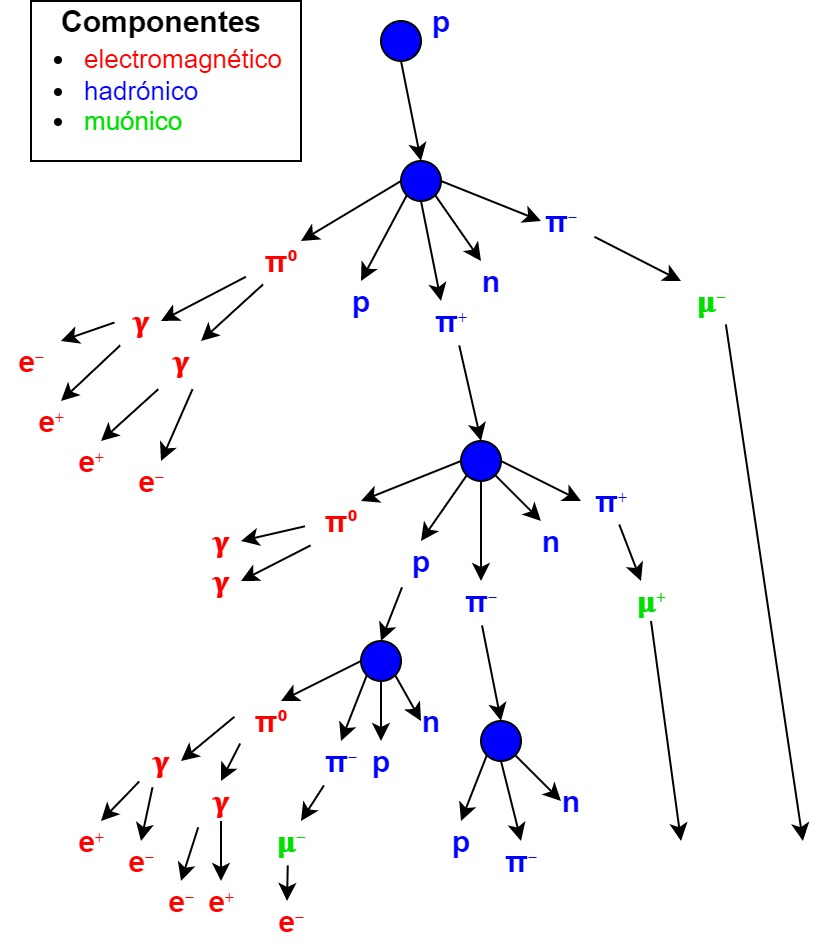
\includegraphics[width=50mm,scale=0.5]{Figures/showercomponents-jpg.jpg}
    \decoRule
    \caption[showercomponents]{caption figure 1}
    \label{fig:showercomponents}
\end{figure}

Los \textbf{rayos cósmicos} son partículas aceleradas en la galaxia o en objetos astrofísicos extragalácticos que al impactar con la atmósfera terrestre generan \textbf{cascadas de partículas} (Figura~\ref{fig:showercomponents}). El consenso general es que rayos cósmicos debajo de energías de 3x10e6 GeV son acelerados en los remanentes de supernovas galácticas y para energías mayores no se tiene una clara idea de que es lo que acelera a estas partículas, lo único que se tiene claro es de que dichas partículas tienen un orígen extragaláctico. A modo de comparación estas fuentes aceleran partículas en tres órdenes de magnitud mayor que el equivalente energético del LHC.

Cuando la energía de los rayos cósmicos sobrepasa significativamente 1000 GeV estos tienen que ser estudiados por las cascadas de partículas que generan en la atmósfera. La mayoría de las cascadas son iniciadas por hadrones con energías que van desde 1000  GeV o mayores a 10 TeV, que al entrar isotrópicamente a la atmósfera producen un gran número de productos secundarios en una serie de colisiones sucesivas con los núcleos de los constituyentes atmosféricos ie. N2, O2, Ar. Estos productos secundarios resultantes se comportan de una manera similar, mientras se van propagando a través de la atmósfera.

Las cascadas de partículas descritas anteriormente son conocidas como \textbf{cascadas atmosféricas extensas} \emph{EAS}. Estas cascadas atmosféricas se propagan longitudinalmente a lo largo de la dirección de incidencia de la partícula primaria, debido al momento transversal de los productos secundarios la cascada también se extiende lateralmente. Como referencia de la complejidad que se tiene, una partícula primaria altamente energética puede crear una cascada gigante de partículas que se propaga esencialmente a la velocidad de la luz a través de la atmósfera y puede alcanzar el nivel del mar si el evento es lo suficientemente energético agregado a lo anterior el número de productos secundarios es del orden 10e10 (Figura~\ref{fig:logitudinaldist}).

\begin{figure}
    \centering
    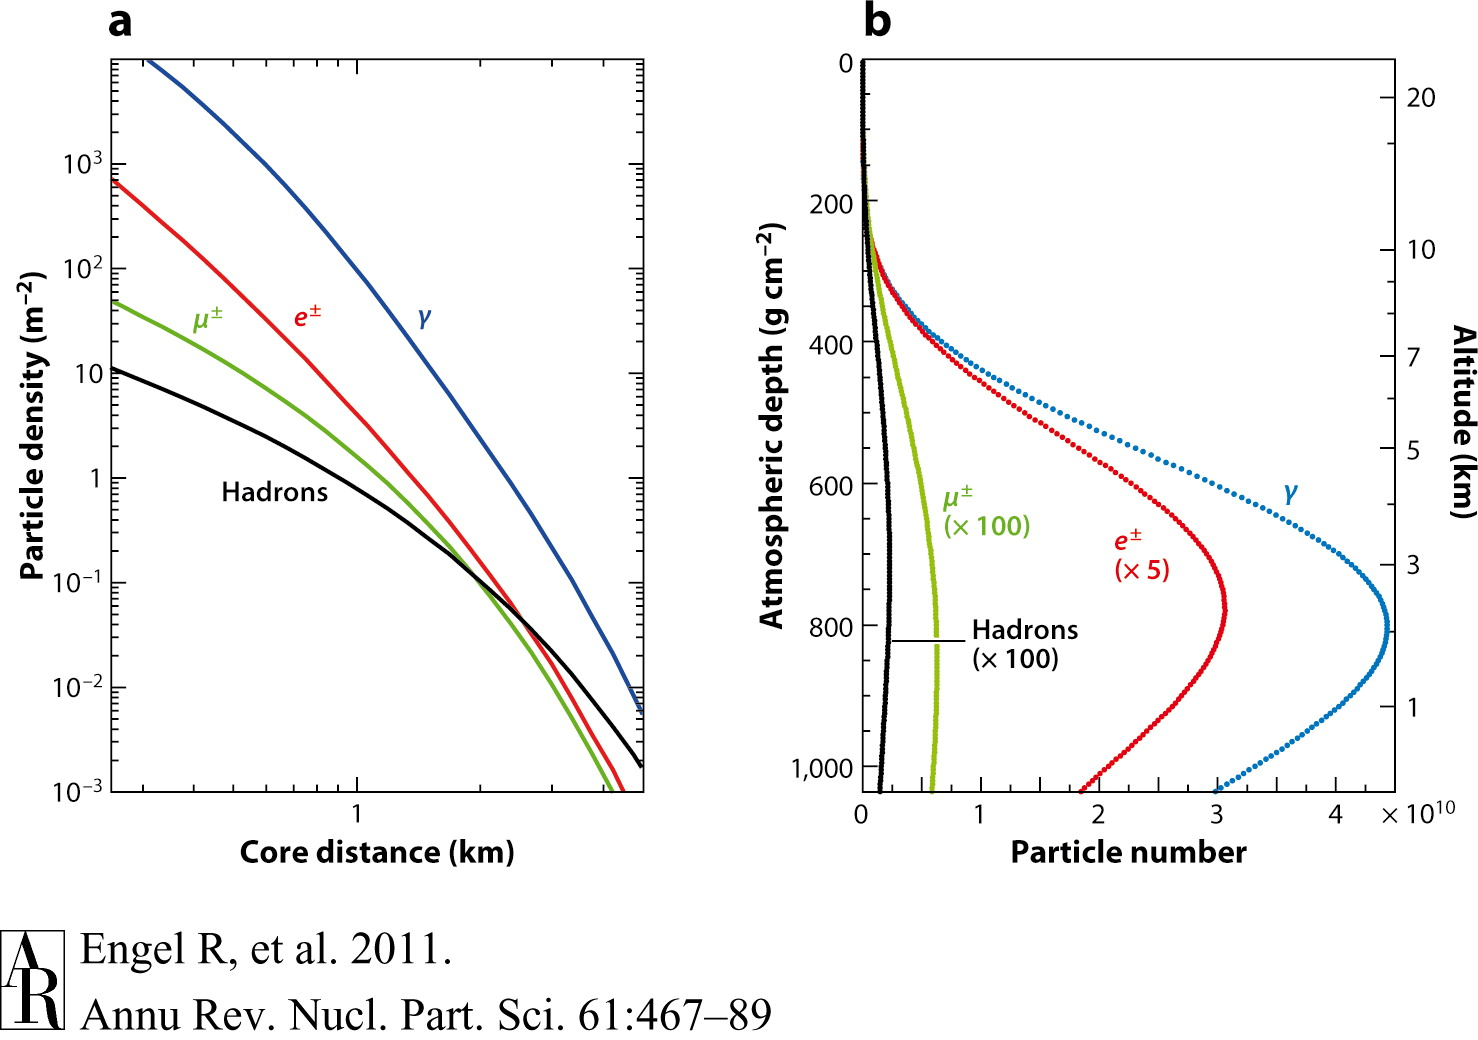
\includegraphics[width=50mm,scale=0.5]{Figures/logitudinaldistribution.jpeg}
    \decoRule
    \caption[logitudinaldist]{caption figure 1}
    \label{fig:logitudinaldist}
\end{figure}

\subsection{Propiedades de las cascadas atmosféricas}

Algunas propiedades que caracterizan a las cascadas atmosféricas son:

\begin{itemize}
    \item \textbf{E0} [eV]: energía de la partícula primaria. 
    \item \textbf{N} (\emph{shower size}): número total de partículas producidas en un nivel en particular de la atmósfera. Es una función que depende de la energía E0, ángulo de incidencia zenith angle y a altura de la primera interacción del evento primario en la atmósfera h1.
    \item \textbf{Xmax} [$gcm^-2$]: profundidad de máximo desarrollo medida desde la parte más alta de la atmósfera. Se desfasa a profundidades mayores conforme la energía del primario se incrementa.
    \item \textbf{Shower Axis}: extensión del vector de momento del primario incidente en la dirección de propagación de la cascada.
    \item \textbf{Dirección de arribo}: dirección de incidencia de la partícula primaria determinada por sus ángulos azimutales y el ángulo zenith.
\end{itemize}

\subsection{Métodos de detección}

Los principales detectores de cascadas atmosféricas son arreglos de detectores espaciados uno del otro en distancias que dependen de la energía de los rayos cósmicos que se quieren observar. Para energías de 10e6 GeV la distancia entre los detectores deben de ser del orden de decenas de metros y para energías que sobrepasan 10e9 GeV la distancia es del orden de miles de metros, por ejemplo en el observatorio Pierre Auger la distancia entre detectores es de 1500m. Diferentes métodos observacionales como detectores de aire cherenkov o detectores de fluorescencia son combinados con estos arreglos como en el caso del observatorio Pierre Auger (Figura~\ref{fig:eas}).

\begin{figure}
    \centering
    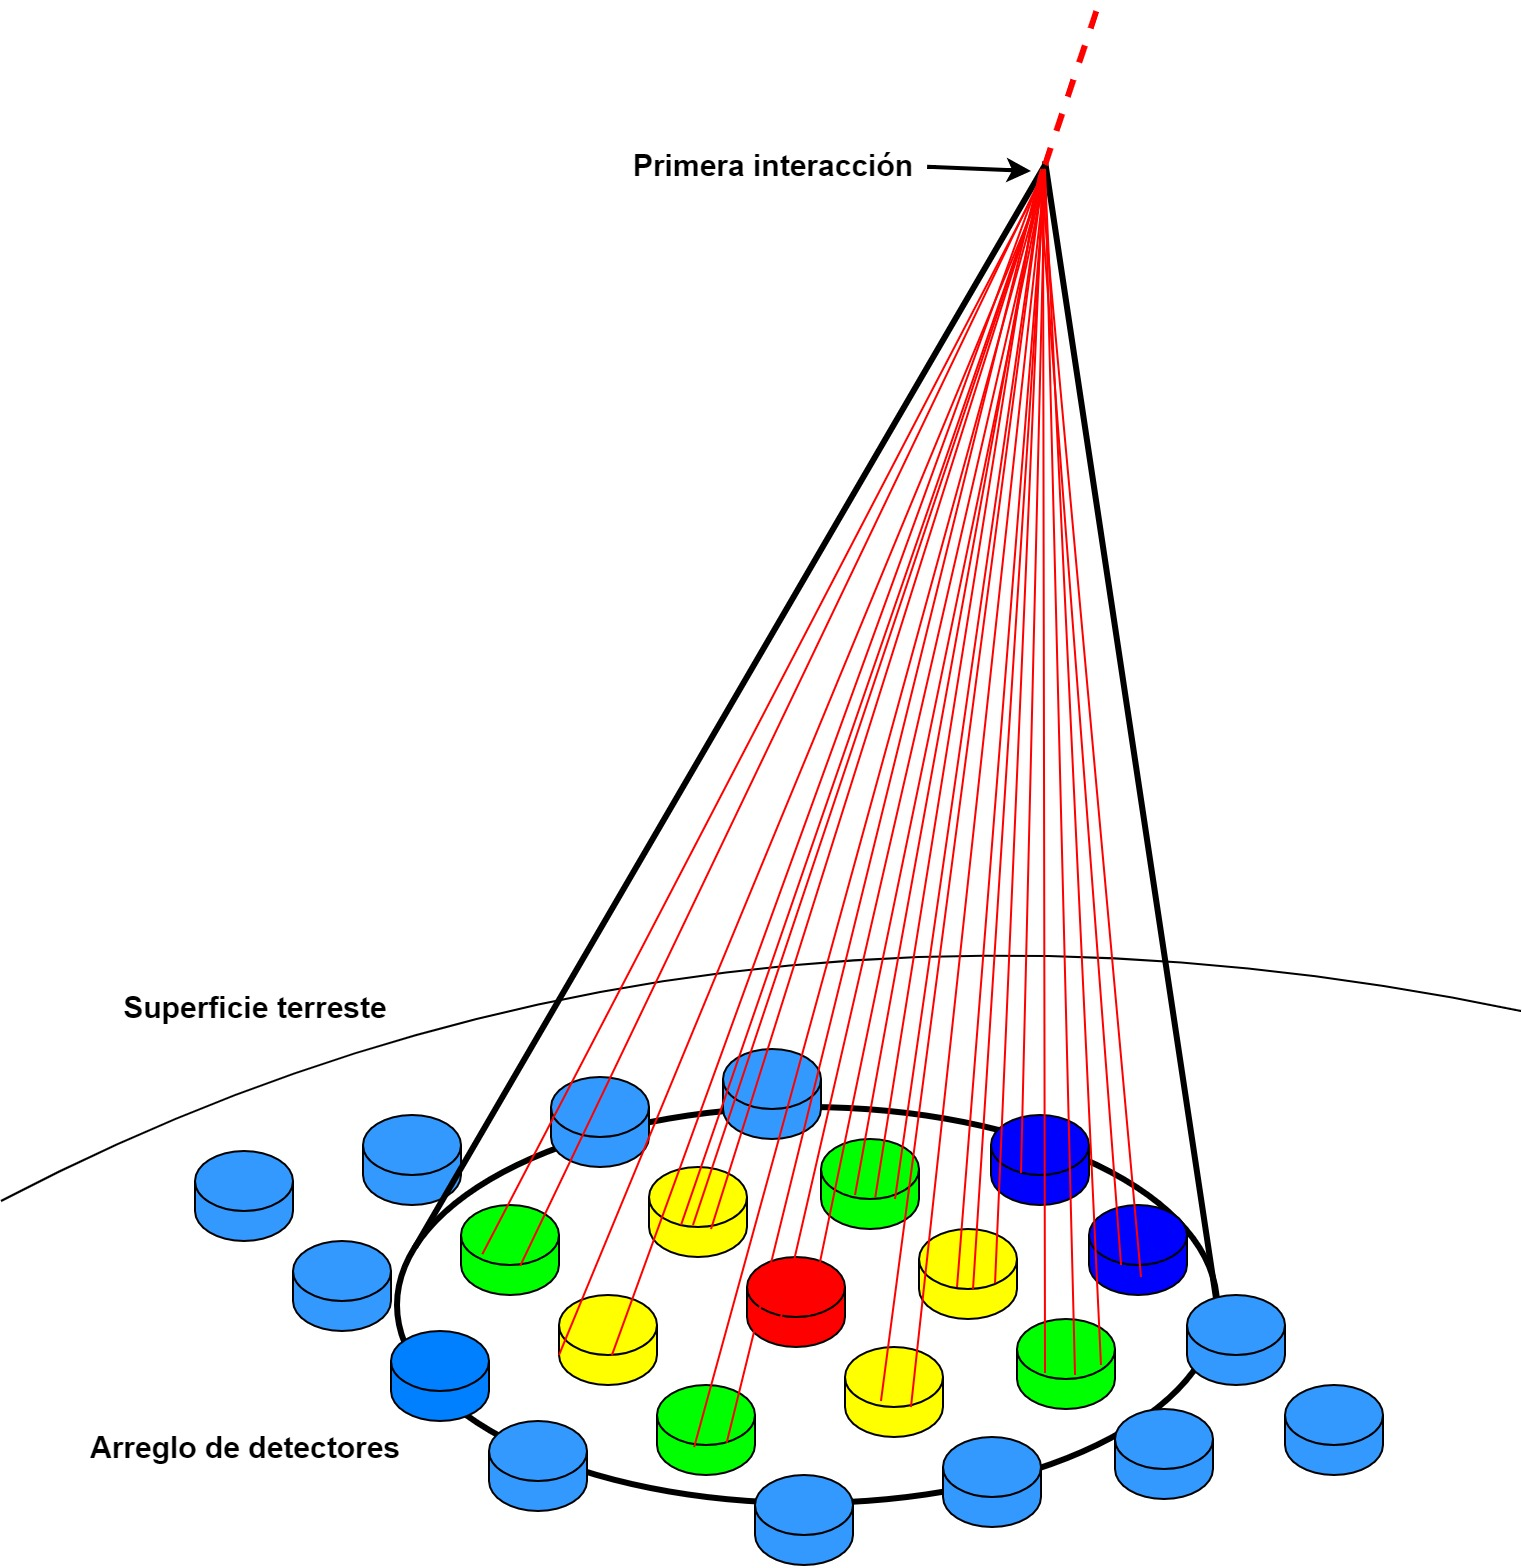
\includegraphics[width=50mm,scale=0.5]{Figures/eas-jpg.jpg}
    \decoRule
    \caption[eas]{caption figure 1}
    \label{fig:eas}
\end{figure}

Sin importar el tipo de sistema de detección que se use, los datos adquiridos representan a la cascada en una etapa en particular de su desarrollo, así como una foto instantánea de la cascada, en el plano de observación. Con estos datos se puede conocer información básica que caracteriza a la cascada atmosférica así como los tiempos de arribo de las partículas cargadas, fotones asociados no ópticos, las distribuciones laterales de partículas y fotones en el plano de observación a una profundidad atmosférica específica. Las propiedades anteriores son inmediatamente accesibles con un arreglo de detectores simple.

La reconstrucción de la partícula primaria depende del modelo hadrónico de interacciones que use el simulador Monte Carlo.

\section{Análisis de las cascadas atmosféricas}

Las cascadas atmosféricas están caracterizadas por un delgado disco de partículas radialmente extenso que se propaga a la velocidad de la luz a través del eje de la cascada. El patrón de las cascadas es circular para cascadas verticalmente incidentes, mientras que la extensión longitudinal y lateral dependen principalmente de la energía de la partícula primaria. El esparcimiento lateral de las partículas en regiones bajas de la atmósfera, llega a cubrir áreas de varios kilómetros cuadrados agregado a lo anterior la mayoría de las partículas arriban en intervalos estrechos de tiempo que van desde unos cuantos nanosegundos en la vecindad del eje de la cascada hasta unos 10 ns a distancias mayores del núcleo de la cascada.

Eventos de baja energía alcanzan su máximo desarrollo en zonas altas de la atmósfera y se mitigan lentamente a mayor profundidad; los componentes que alcanzan a llegar a la superficie son los muones y neutrinos. Para eventos extremadamente energéticos las cascadas logran alcanzar su máximo desarrollo a nivel del mar mientras que sus componentes hadrónicos y electromagnéticos sobrevivientes, son absorbidos en la superficie terrestre y los muones resultantes altamente energéticos continúan propagándose bajo tierra. 

Como regla de dedo se puede decir que en promedio una cascada atmosférica está constituida al $1\%$ por hadrones, alrededor del $10\%$ son muones y el $90\%$ o más son electrones o positrones. También para las primeras estimaciones energéticas de la primaria, se tiene que cascadas verticales a una altitud de 5km tienen una energía $~1$ GeV, $~3$ GeV para alturas entre 2.5 km y 3 km $~10$ GeV a nivel del mar.

\begin{figure}
    \centering
    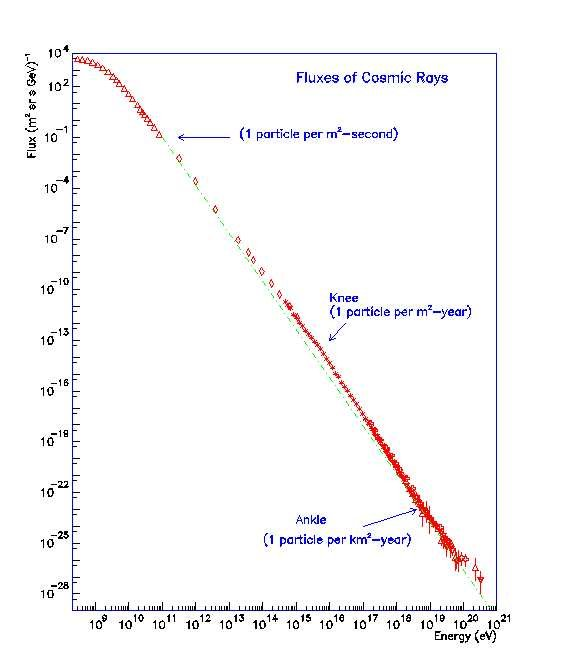
\includegraphics[width=50mm,scale=0.5]{Figures/All-particle-cosmic-rays-energy-spectrum.jpg}
    \decoRule
    \caption[energyspectrum]{caption figure 1}
    \label{fig:energyspectrum}
\end{figure}

Para poder visualizar la ocurrencia de estos eventos en distintos regímenes energéticos se puede estudiar el número de partículas que cruzan un área en un tiempo dado, conocido como flujo cósmico. Este flujo sigue una ley de potencias con la forma $\frac{1}{E^3}$, en se puede ver  energías alrededor de $10^12$ eV el flujo es de 10 partículas primarias por minuto y $m^2$, para energías entre $10^18$ eV y $10^19$ eV se tiene 1 partícula primaria por año y $km^2$ en estos regímenes energéticos las estadísticas son pobres y las incertidumbres altas. 

Los observables importantes que se deben de obtener para poder reconstruir una cascada son, el tiempo de arribo $t_i$ al detector $i$ respecto al tiempo de referencia $t_0$, la densidad de partículas $\rho_i$ y la posición del detector con respecto al sistema de referencia $(x_i, y_i)$.
Con la distribución lateral de las partículas su puede adquirir la localización del eje de la cascada y el tamaño de la cascada para así obtener un estimado de la energía. Los parámetros anteriores son clasificados como accesibles directamente ya que no necesitan un análisis complejo para su adquisición. 

Por último, parámetros indirectamente accesibles que se relacionan con la naturaleza de la partícula primaria, como el tipo de partícula, masa y carga, no se pueden extraer inmediatamente y requieren métodos sofisticados de análisis. 

La mayoría de las partículas arriban en intervalos estrechos de tiempo que van desde unos cuantos nanosegundos en la vecindad del eje de la cascada hasta unos 10 ns a distancias mayores del núcleo de la cascada.

\section{Simulaciones}

Simuladores de cascadas atmosféricas son de vital importancia para la evaluación e interpretación de datos experimentales. Las técnicas se reducen a crear e insertar un modelo de cascadas que corresponda a nuestro mejor entendimiento de la realidad, simular cascadas, comparar resultados con los datos experimentales, modificar el modelo o sus parámetros y intentar de nuevo; hacer ajustes pequeños al modelo y repetir hasta que se obtenga un consenso entre la predicción y el experimento.

Las cascadas iniciadas por primarios hadrónicos consisten en la superposición de dos tipos de cascadas, una hadrónica y otra electromagnética. La cascada electromagnética se entiende bien y solo posee problemas prácticos asociados al gran número de partículas participantes en el orden de $~10^10$. Los programas computacionales que simulan cascadas hadrónicas o electromagnéticas de alta energía o cascadas atmosféricas completas son altamente complejos.

Para tomar en cuenta la complejidad computacional que se tiene, una simulación completa de una cascada debe incluir los componentes electromagnéticos y hadrónicos. Además se debe de tomar en cuenta todos los procesos relevantes, donde la mayoría son de naturaleza estocástica y muchos están en competencia entre sí. También se debe incluir los parámetros que especifican el estado de cada partícula como su masa, carga, energía, momento, ubicación de su creación en el espacio tiempo x,y,z,t, la orientación angular respecto al marco de referencia y parámetros genéticos que revelan la altura de la interacción donde cada partícula fue creada. Estos observables son cruciales para análisis subsecuentes y para la comparación con datos experimentales.

\subsection{Estrategia para simulaciones de EAS}

La arquitectura del sistema ASICO sirve como base para entender el proceso de un simulador completo. ASICO fue el primer simulador que generaba cascadas detalladas al usar 12 parámetros que definen a cada partícula y este fue la base para el desarrollo de CORSIKA.
Para simular una cascada completa se comienza con la simulación de la cascada hadrónica y se le llama PASO 1, este paso da lugar a datos como la elasticidad, distribuciones de interacciones hadrónicas en diferentes rangos de energías, entre otros; para la parte electromagnética de la cascada se le llama PASO 2 y la combinación de las dos simulaciones para formar la cascada completa se le conoce como el PASO 3.

\begin{figure}
    \centering
    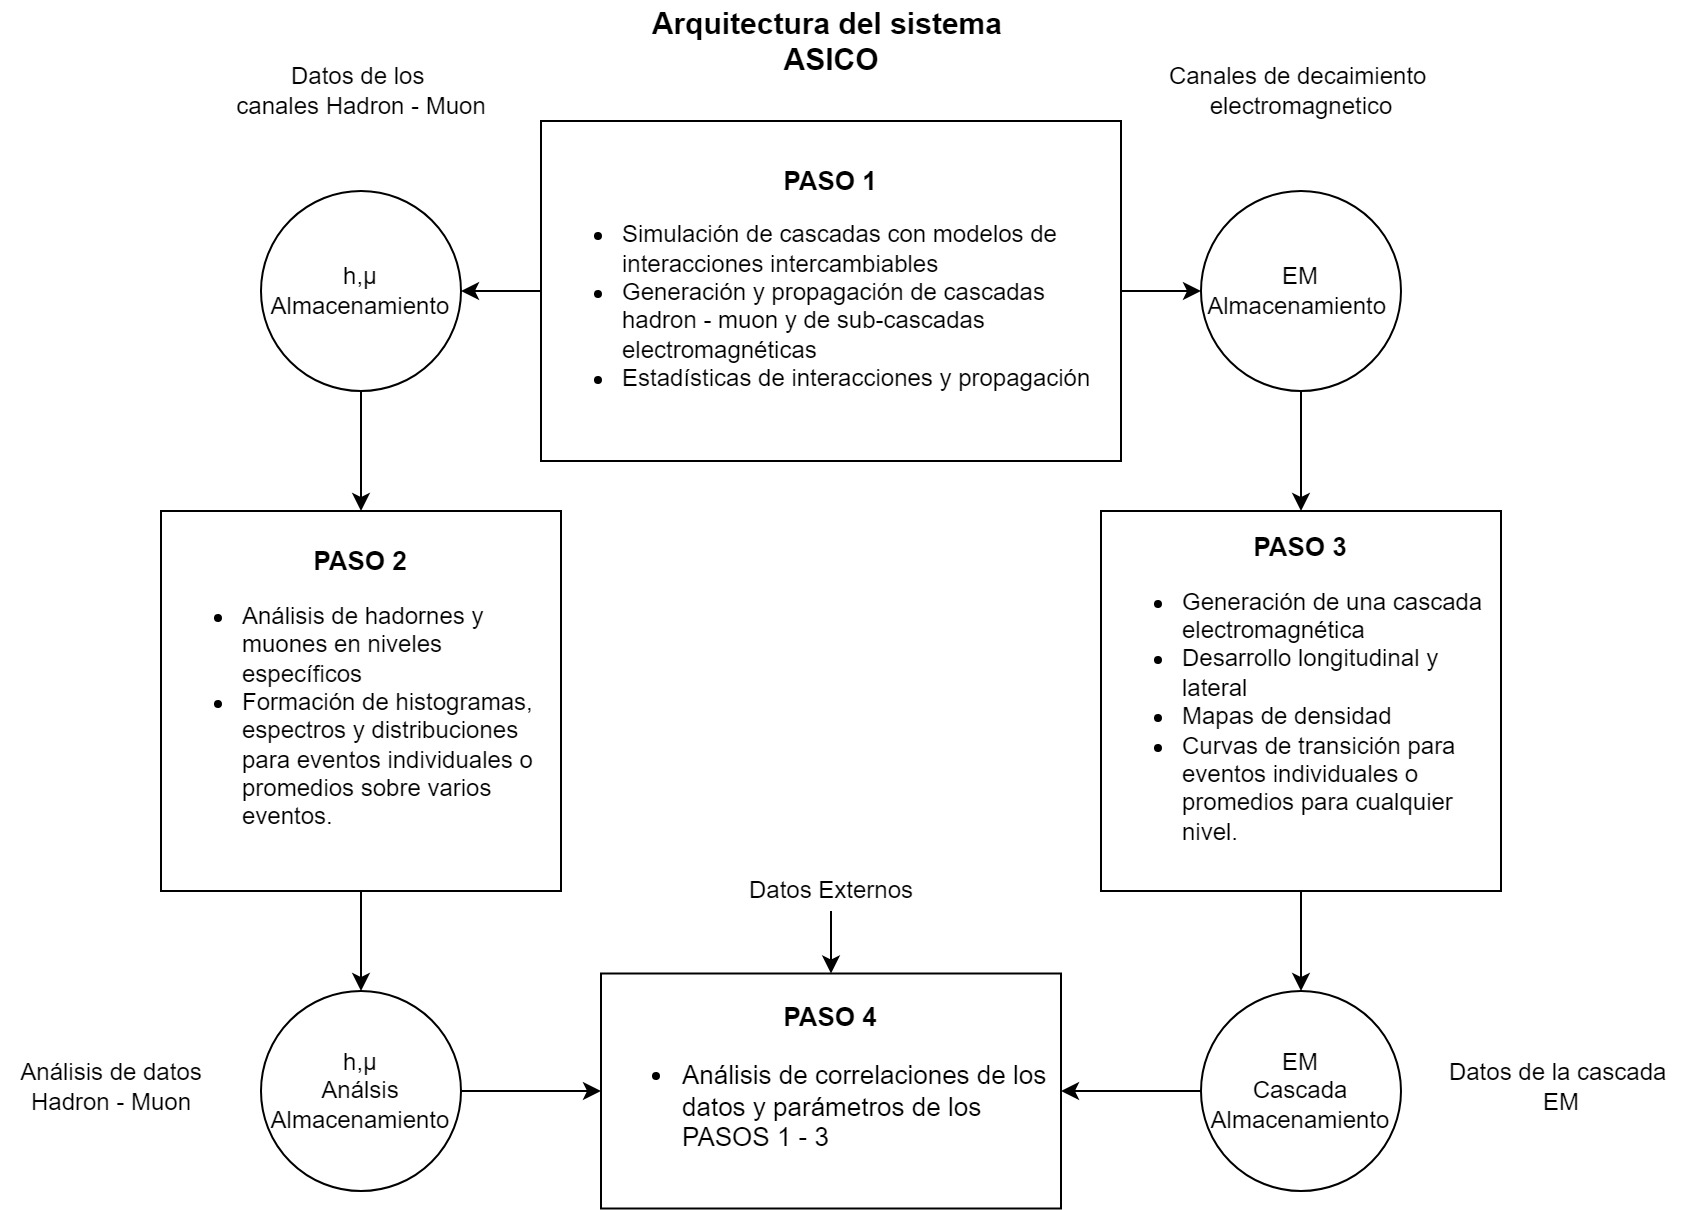
\includegraphics[width=50mm,scale=0.5]{Figures/asico-jpg.jpg}
    \decoRule
    \caption[asicoarq]{caption figure 1}
    \label{fig:asicoarq}
\end{figure}

% Hablar un poco más sobre cómo se usa Monte Carlo en los simuladores

\subsection{Problemática de las simulaciones}

Los parámetros que determinan a cada partícula se deben de asignar en su punto de creación y requieren actualizarse después de cada proceso al cual está sujeta. Esto es al final de cada trayectoria particular, después de propagarse al siguiente punto de interacción o decaimiento y cuando pasan a un nuevo nivel de observación. En cada actualización la partícula y sus parámetros son guardados para su subsecuente análisis y evaluación de los datos de la cascada simulada.

Consecuentemente, la ejecución de programas que simulan cascadas requieren mucho tiempo computacional  particularmente para cascadas energéticas donde el número de partículas involucradas se vuelve muy grande. La gran cantidad de datos producidos por estas simulaciones requieren también una gran capacidad de almacenamiento. La complejidad aumenta si los componentes atmosféricos cherenkov o de fluorescencia se incluyen, en este caso los datos corren el riesgo de divergir y métodos computacionales más sofisticados deben de ser usados para su análisis.

En general el desarrollo y la propagación de una cascada a partir del punto de iniciación (la primera interacción) hasta  el nivel de observación consume más tiempo que el análisis subsecuente de los datos producidos.

\begin{itemize}
    \item \textbf{Memoria:} Almacenamiento confiable de los datos crudos.
    \item \textbf{Rastreabilidad:} Rastreo de los parámetros que determinan a cada partícula.
    \item \textbf{Fenomenología:} Propagación de las partículas en la atmósfera tomando en cuenta todos los procesos a los que están sujetas.
    \item \textbf{Configuración inicial:} Correlación confiable entre los parámetros iniciales ( \emph{i.e.} modelos de interacción, propiedades del detector, propiedades de la primaria) con la cascada final
    \item \textbf{Tiempo:} Existe una relación lineal entre la energía de la partícula y el tiempo que lleva simular la cascada que genera.
\end{itemize}

\section{Modelos generativos}

Los modelos generativos son un tipo de aprendizaje no supervisado, que describen cómo se genera un conjunto de datos en términos de un modelo probabilístico. Al muestrear de dicho modelo se es capaz de generar datos no observados previamente. Típicamente el marco de trabajo de los modelos generativos involucra las siguientes partes.

\begin{itemize}
    \item \textbf{Los datos:} Conjunto de observaciones, que se asumen ser generadas de acuerdo a una distribución de probabilidad desconocida.
    \item \textbf{El modelo:} Un modelo generativo que intenta imitar lo mejor posible, a la distribución que genera las observaciones. Este modelo es capaz de generar datos no observados que parecen haber sido generados con la distribución desconocida y no debe de generar datos conocidos.
\end{itemize}

\subsection{Aplicación de modelos generativos}

Algunas de las tareas modernas de los modelos generativos son:

\begin{itemize}
    \item \textbf{Generación de datos novedosos:} Se generan datos nunca antes vistos que pueden ser utilizados para imitar fenómenos o para ayudar a flujos en modelos discriminativos con un pre entrenamiento autosupervisado.
    \item \textbf{Compresión de datos:} El modelo es capaz de aprender las características más importantes que determinan a la observación y así logra reducir la dimensionalidad del espacio de características donde vive la observación original. 
    \item \textbf{Tecnologías de síntesis condicional:} Proporciona un método capaz de generar información novedosa condicionada a un dominio específico. Lo anterior permite una suerte de transformación de datos de un dominio a otro. 
\end{itemize}

Las tareas anteriores han logrado avances en:

\begin{itemize}
    \item Generacion de rostros humanos
    \item Transformación de imágenes
    \item Transferencia de estilos
    \item Texto a imagen
    \item Texto a voz
    \item Edicion de imagenes
    \item Super resolución
    \item Generación de objetos 3D
    \item Predicción de fotogramas en videos
\end{itemize}